%%%%%%%%%%%%%%%%%%%%%%%%%%%%%%%%%%%%%%%%%
% Journal Article
% LaTeX Template
% Version 1.3 (9/9/13)
%
% This template has been downloaded from:
% http://www.LaTeXTemplates.com
%
% Original author:
% Frits Wenneker (http://www.howtotex.com)
%
% License:
% CC BY-NC-SA 3.0 (http://creativecommons.org/licenses/by-nc-sa/3.0/)
%
%%%%%%%%%%%%%%%%%%%%%%%%%%%%%%%%%%%%%%%%%

%----------------------------------------------------------------------------------------
%	PACKAGES AND OTHER DOCUMENT CONFIGURATIONS
%----------------------------------------------------------------------------------------

\documentclass[twoside]{article}

\usepackage{lipsum} % Package to generate dummy text throughout this template

\usepackage[sc]{mathpazo} % Use the Palatino font
\usepackage[T1]{fontenc} % Use 8-bit encoding that has 256 glyphs
\linespread{1.05} % Line spacing - Palatino needs more space between lines
\usepackage{microtype} % Slightly tweak font spacing for aesthetics

\usepackage[hmarginratio=1:1,top=32mm,columnsep=20pt]{geometry} % Document margins
\usepackage{multicol} % Used for the two-column layout of the document
\usepackage[hang, small,labelfont=bf,up,textfont=it,up]{caption} % Custom captions under/above floats in tables or figures
\usepackage{booktabs} % Horizontal rules in tables
\usepackage{float} % Required for tables and figures in the multi-column environment - they need to be placed in specific locations with the [H] (e.g. \begin{table}[H])
%\usepackage{hyperref} % For hyperlinks in the PDF

\usepackage{lettrine} % The lettrine is the first enlarged letter at the beginning of the text
\usepackage{paralist} % Used for the compactitem environment which makes bullet points with less space between them

\usepackage{abstract} % Allows abstract customization

\renewcommand{\abstractnamefont}{\normalfont\bfseries} % Set the "Abstract" text to bold
\renewcommand{\abstracttextfont}{\normalfont\small\itshape} % Set the abstract itself to small italic text

\usepackage{titlesec} % Allows customization of titles
\renewcommand\thesection{\Roman{section}} % Roman numerals for the sections
\renewcommand\thesubsection{\Roman{subsection}} % Roman numerals for subsections
\titleformat{\section}[block]{\large\scshape\centering}{\thesection.}{1em}{} % Change the look of the section titles
\titleformat{\subsection}[block]{\large}{\thesubsection.}{1em}{} % Change the look of the section titles

\usepackage{fancyhdr} % Headers and footers
\usepackage{graphicx}
\pagestyle{fancy} % All pages have headers and footers
\fancyhead{} % Blank out the default header
\fancyfoot{} % Blank out the default footer
%\fancyhead[C]{Running title $\bullet$ November 2012 $\bullet$ Vol. XXI, No. 1} % Custom header text
\fancyhead[C]{CS229 Final Paper} % Custom header text
\fancyfoot[RO,LE]{\thepage} % Custom footer text

\newenvironment{Figure}
{\par\medskip\noindent\minipage{\linewidth}}
{\endminipage\par\medskip}
%----------------------------------------------------------------------------------------
%	TITLE SECTION
%----------------------------------------------------------------------------------------

\title{\vspace{-15mm}\fontsize{24pt}{10pt}\selectfont\textbf{Predicting Sales for Rossmann Drug Stores}} % Article title

\author{
\large
\textsc{Brian Knott, Hanbin Liu, Andrew Simpson}\\[2mm] % Your name
%\normalsize \href{mailto:john@smith.com}{john@smith.com} % Your email address
\vspace{-5cm}
}
\date{}

%----------------------------------------------------------------------------------------

\begin{document}

\maketitle % Insert title

\thispagestyle{fancy} % All pages have headers and footers

%----------------------------------------------------------------------------------------
%	ABSTRACT
%----------------------------------------------------------------------------------------
\vspace{-1cm}
\begin{abstract}

%\noindent \lipsum[1] % Dummy abstract text
\noindent In this paper we examined four different methods for time series forecasting: Random Forests, Gradient Boosting, Hidden Markov Models, and Recurrent Neural Networks. We found that using Gradient Boosting yielded the best results with root-mean-square percent error (RMPSE) of 10.439\% (785 of 3429). 

\end{abstract}

%----------------------------------------------------------------------------------------
%	ARTICLE CONTENTS
%----------------------------------------------------------------------------------------

\begin{multicols}{2} % Two-column layout throughout the main article text

\section{Introduction}

\lettrine[nindent=0em,lines=3]{T} he goal of Rossmann Kaggle competition is to forecast the daily sales of Rossmann stores located across Germany using store, promotion, and competitor data. It is known that store sales are influenced by many factors, including promotions, competition, school and state holidays, seasonality, and locality. A reliable and robust prediction model will enable store managers to create effective staff schedules that increase productivity. The data are provided by Rossmann through Kaggle.

%------------------------------------------------

\section{Related Work}
\indent \indent The models we use in this paper have been widely studied. The framework for Gradient Boosting is laid out in [3] and [4], Random Forests are studied in [2], Recurrent Neural Networks in [5], and Hidden Markov Models in [6]. These papers describe how parameters effect model prediction. \\
\indent  Additionally, 3429 groups have submitted results to this Kaggle competition. The code for many of these submission is available on the competition's Scripts page. The majority of the submissions used Random Forest or Gradient Boosting approaches, likely because there are reliable packages for their implementation. Results of these approaches vary widely, however, due to different choices in parameters, preprocessing, and data splitting.



%------------------------------------------------

\section{Dataset and Features}


\indent \indent Rossmann provided data with 15 features for 1115 stores. Not all stores have data for each feature on each day, so we filled in missing data with median data for non-ensemble methods (ensemble methods did not require data for every field). We then extended the data to 18 features since some features, like the date, captured multiple variables (like month of the year and day of the month). The resulting data had the following feature set: \\

\begin{table}[H]
\caption{Feature Set}
\centering
\begin{tabular}{ll}
\toprule
\cmidrule(r){1-2}
Feature ID & Description \\
\midrule
1 &  Store ID \\
2 &  Day Of Week \\
3 & Open / Closed\\
4 &  Promotion Active \\
5 & School Holiday\\
6 & Store Type \\
7 & Assortment \\
8 & Distance to Competing Store\\
9 & Month Competitor Opened \\
10 & Year Competitor Opened\\
11 & Promo2 Active \\
12 & Week Promo2 Started\\
13 & Year Promo2 Started\\
14 & Interval of Promo2\\
15 & Month \\
16 & Year \\
17 & Day \\
18 & Competition Age (GB only)\\
\bottomrule
\end{tabular}
\end{table}

\noindent We then normalized the data to have zero mean before applying our learning algorithms.



%------------------------------------------------

\section{Methods}

\subsection{Random Forests}

Random Forest Regression is an ensemble learning algorithm that operates by aggregating many random decision trees to make predictions while avoiding overfitting. We started by using the Random Forest algorithm for black box prediction because its bagging techniques are robust to data anomalies (like missing data) and because random forest packages are widely available.

In particular, we used R's RandomForest package to carry out the training and prediction. We then used parameter optimization to improve on our prediction model. To see our parameter optimization method (and the parameters used) see the Results section.

\subsection{Hidden Markov Models}
Hidden Markov Modeling is a sequence / state estimation algorithm that assumes that the dataset derives from a Markov Process with hidden state information. Hidden Markov Models are appropriate for this dataset since its data evolves over time, a phenomenon unaccounted for in ensemble learning.
\vspace{-1mm}
\begin{equation}
P(z_{t}|z_{t-1},z_{t-2},...z_{1})=P(z_{t}|z_{t-1})
\label{eq:hmmLimited}
\end{equation}

Hidden Markov models rely on two sets of Markov assumptions. The first is the limited horizon assumption. This assumes that the probability of being in a state depends only on the most recent states. For a first order Markov model, the current state \begin{math}z_{t}\end{math} depends only on the state \begin{math}z_{t-1}\end{math} (Eq. 1).

The second assumption is that the state transition process is stationary. This means that the conditional distribution of state transitions does not change over time (Eq. \ref{eq:hmmStationary}).

\vspace{-1mm}

\begin{equation}
P(z_{t}|z_{t-1}) = P(z_{2}|z_{1});t\in 2...T
\label{eq:hmmStationary}
\end{equation}


The transition between states can be estimated by averaging the number of times a state transitioned from another stated. We used Laplace smoothing to replace zero probabilities with a small probabilities (Eq. \ref{eq:hmmlaplace} where \begin{math}k\end{math} = number of states).

\vspace{-1mm}

\begin{equation}
\hat{p}({s_{i}|s_{j}}) = \frac{\sum_{t=1}^{T}1\{z_{t-1} = s_{i} \wedge z_{t} = s_{j}\}+1}{\sum _{t=1}^{T}\{ z_{t-1} = s_{i}\} + k}
\label{eq:hmmlaplace}
\end{equation}

A hidden Markov model is made of two sets of states one hidden and the other observed. We want to find the most likely series of hidden states given the observed states and known transitions between the observed states and the hidden states. This can be done naively by keeping track of all the provabilities; however, this is computationally expensive. A dynamic programing approach, known as the Viterbi algorithm, is used instead. This algorithm instead keeps track only of the maximum probabilities through a recursive definition.



\subsection{Recurrent Neural Networks}
\indent \indent Recurrent Neural Networks work similarly to standard artificial neural networks with the addition of feedback loops. The internal recursive states allow this kind of neural network to exhibit dynamic temporal behavior, making it appropriate for processing time series data.

\indent A neuron is made up of two parts a weighted sum (weights, inputs, and a bias) and an activation function. In order to learn on non-linear data, the hidden layer neurons usually use an activation function that is in the sigmoid family (logistic, Gaussian, etc.). The output of each neuron is the weighted sum passed into the activation function. The output of each neuron is passed to each neuron in the next layer. When predicting a continuous value, a single linear output neuron is usually used. Learning is usually done on neural networks through the back propagation algorithm. This algorithm splits the error (squared error) between each weight it the network. In order to do this, we use the chain rule. On the hidden layers the sum of the derivative is part of the chain that is multiplied to find the error. An example of how error flows back to the hidden layer is given in Eq. \ref{eq:backprop} (net is net sum of weights times inputs and bias).

\begin{figure*}[!t]
\begin{center}
\begin{equation}
\frac{\partial Error_{total}}{\partial w_{hidden}} = \left ( \sum_{Higher Layer}\frac{\partial Error_{total}}{\partial output_{higher}}*\frac{\partial output_{higher}}{\partial net_{higher}}*\frac{\partial net_{higher}}{\partial output_{hidden}} \right )*\frac{\partial output_{hidden}}{\partial net_{hidden}}*\frac{\partial net_{hidden}}{\partial w_{hidden}}
\label{eq:backprop}
\end{equation}
\vspace*{4pt}
\end{center}
\end{figure*}





In recurrent neural networks the output of the hidden layer neurons feeds back as another input. A basic layout of a recurrent neural network is given in figure \ref{fig:RNNExample}. Since the input from the previous time is passed as input to the current time, recurrent neural networks have a form of memory. With a recursive definition, this memory covers every input set.


 \begin{Figure}
	 \centering
	 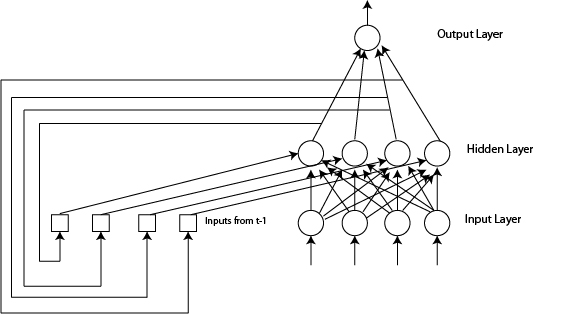
\includegraphics[width=\linewidth]{images/RNN.jpg}
	 \captionof{figure}{An example recurrent neural network. Outputs from the hidden layer neurons from the previous time step are fed back in as input to the next time step.}
	 \label{fig:RNNExample}
 \end{Figure}


\subsection{Gradient Boosting Regression}

\indent \indent Gradient Boosting is an ensemble learning algorithm that uses a weighted average of simple models to learn a more complex model. The algorithm first uses a simple model to fit the data, then a simple model to fit the residuals between the data and the first model. This process continues on each model's residuals until an appropriate fit is found. \\
As the model increases in complexity, overfitting tends to start occurring. To avoid overfitting, the Gradient Boosting algorithm keeps a portion of the data (different in each iteration) out of the training set and uses it for cross validation. The algorithm keeps track of the cross validation error and determines that an appropriate fit has been found once the cross validation error increases for a given number of iterations. \\
\indent We used the R package XGBoost to train our Gradient Boosting models, then used parameter optimization to find the best solution.


\section{Results and Discussion}

\subsection{Random Forest}

\indent \indent For our Random Forest approach, we used the R package RandomForest for training models and making predictions. This package allows for the variation of three major parameters. Each parameter is mainly used to balance the tradeoff between runtime and fit quality. Because random forest regression is a very resource hungry algorithm, parameters must be set with feasibility in mind. The parameters given to the model are as follows:
\begin{itemize}
\item \textit{mtry} - the number of features allowed in each decision tree. For a given value $k$, trees may not use more than $k$ regressor variables from the 18 features given to the model. Higher values for \textit{mtry} allows each tree to model more information from the features, but requires more trees to generate an informative average.
\item \textit{ntrees} - the number of trees averaged in the model. A higher value means runtime will be longer, but with a better fit.
\item \textit{sample size} - because the training algorithm is so resource hungry and Rossmann provided so much data, it is not feasible to run Random Forest Regression on the whole dataset. Therefore this parameter sets the number of random data samples that the model is trained on. 
\end{itemize}

Table 2 shows the parameters for our best two Random Forest models as well as the prediction RMSPE as scored by Kaggle (Kaggle scores on data for which we only have access to the feature data).

\begin{table}[H]
\caption{Parameter Selection for Random Forest Regression}
\centering
\begin{tabular}{lccr}
\toprule
\cmidrule(r){1-4}
\textit{mtry} & \textit{ntrees} & \textit{samplesize} & RMSPE\\
\midrule
7 &  100 & 100000& 12.09\% \\
9 &  300 & 100000& 11.98\%\\

\bottomrule
\end{tabular}
\end{table}


\subsection{Hidden Markov Model}

\begin{Figure}
    \centering
    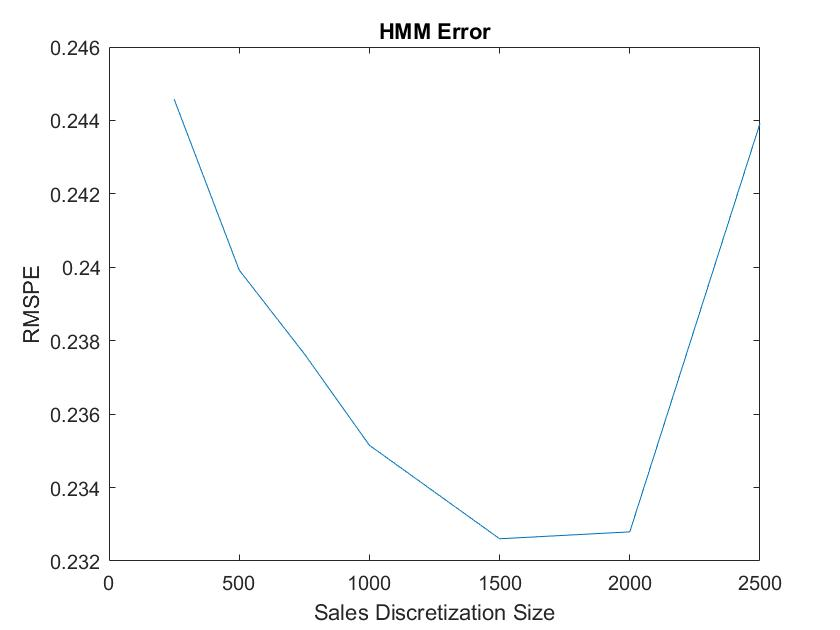
\includegraphics[width=\linewidth]{images/learningSmoothLabelHMM.jpg}
    \captionof{figure}{HMM error using Laplace Smoothing}
    \label{fig:hmmSmooth}
\end{Figure}

For testing with HMMs, the stores were treated separately. The decision to use the stores separately came from An experiment normalizing the data to zero mean and combining the stores to estimate transitions. Combining all this produced a much higher error (over 70\% RMSPE) and was computationally expensive.

The observed states, what we know in advance, is everything except sales and customer data. There are 224 state for different observations (7 days in a week, Store Open/Closed, Promotion Active, 4 state holidays, and a school holiday). The sales data needed to be discretized to work with the hidden Markov model. A smaller discretization leads to the potential ability to be close to the true value; however, it also decreases the probability estimation between states as there are more states. Figure \ref{fig:hmmSmooth} show the results of different levels of sales discretization. This experiment showed that dividing sales by 1500 and rounding produced the lowest training error.

\begin{Figure}
    \centering
    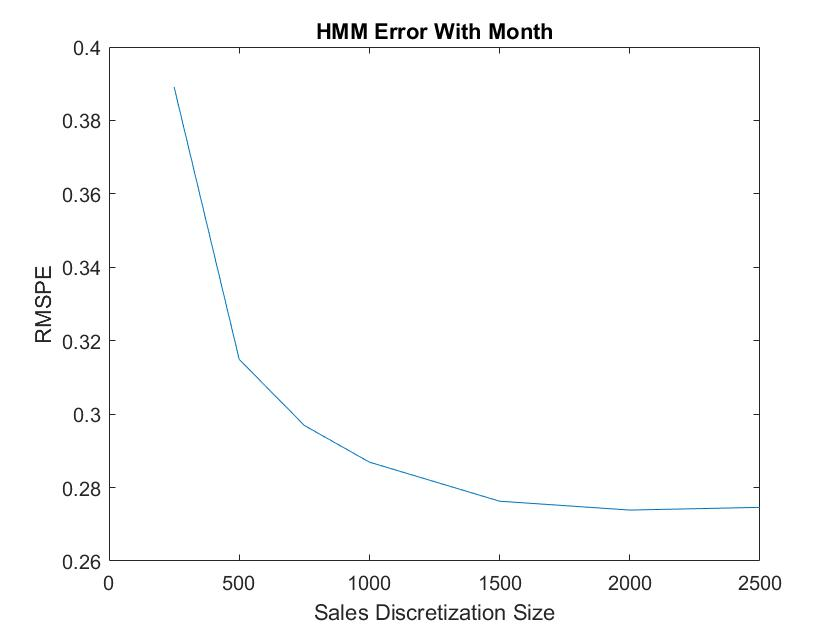
\includegraphics[width=\linewidth]{images/learningWithMonthLabelHMM.jpg}
    \captionof{figure}{HMM error using Laplace Smoothing and month data}
    \label{fig:hmmSmoothMonth}
\end{Figure}


In order to account for seasonality effects, the month was also included as an experiment. However, when tested the training error was higher than not including this data (see figure \ref{fig:hmmSmoothMonth}). Increasing the number of observed states by a factor of 12 (2688 states) likely decreased the estimation of state transitioning.





\subsection{Recurrent Neural Network}

\indent \indent Due to the temporal nature of the data hold out cross validation was used. 20\% of the data was left out for validation. In order to work with the Matlab's functionality, the data was normalized. Each store was treated separately for reasons similar to the Hidden Markov method. During testing it was found that the predicted values for closed days did not always go to zero, so we set values for closed days to zero. An experiment was to test the effect the different numbers of neurons had in the hidden layer. The experiment show that 7 neurons produced the lowest training error (see figure \ref{fig:RNNErrorForceZero}).

\begin{Figure}
    \centering
    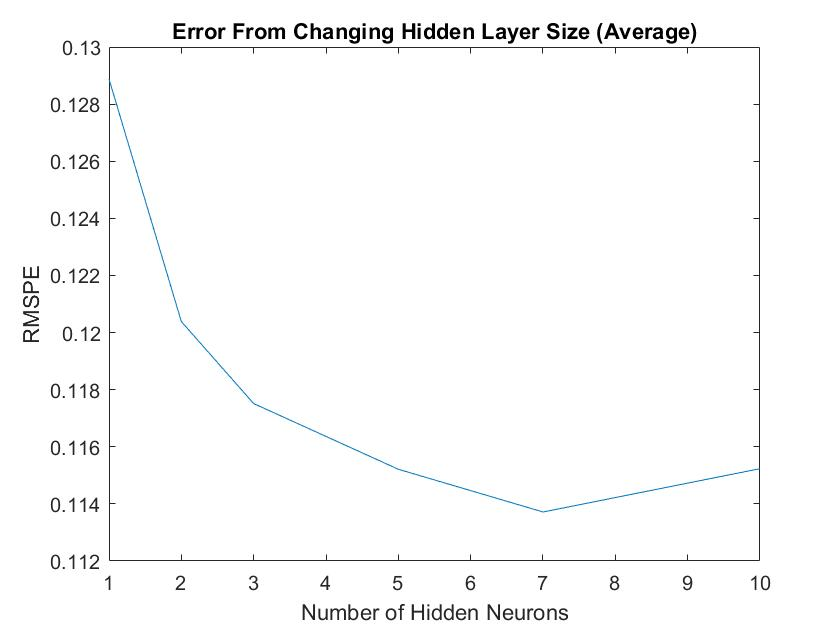
\includegraphics[width=\linewidth]{images/hiddenAverageForceZero.jpg}
    \captionof{figure}{RNN Error averages of different number of hidden neurons (closed days forces to 0).}
    \label{fig:RNNErrorForceZero}
\end{Figure}

The actual error from Kaggle had much higher error of around 24\%. This may be due to over fitting. The neural network may have learned the pattern leading up to the test date, but the Kaggle test data started at a different time.

\subsection{Gradient Boosting}
\indent \indent Similar to Random Forests, Gradient Boosting is an ensemble based regression, efficient for black-box prediction. However, Gradient Boosting is much faster to train than Random Forests. It has been used in several Kaggle competition-winning solutions and has been developed into a the R package XGBoost. \\
\begin{table}[H]
\caption{Model Performance}
\begin{tabular}{lccr}
\toprule
\cmidrule(r){1-4}
 \textit{ntrees} & \textit{Parallel Trees} & \# Features & RMSPE \\
\midrule
3000 & default(1) & 17 & 10.68\% \\
5000 & default(1) & 17 & 10.70\% \\
3000 & 10 & 17 & 10.52\% \\
3000 & 10 & 17 & 10.50\% \\
3000 & default(1) & 18 & 10.58\% \\
3000 & 10 & 18 & 10.56\% \\
\bottomrule
\end{tabular}
\end{table}

\indent As shown in Table 3, our first run of Gradient Boosting generated a RMSPE of 10.681\%, a significant improvement on our best Random Forest model. To further improve our model, we increased the number of trees from 3000 to 5000, however the model wight 5000 trees performed worse than the previous model. We believe this to be due to overfitting since the cross-validation error does not improve from 3000 to 5000 trees while the training error goes down (as seen in Figure 5). Therefore, we chose to keep the number of trees set at 3000. We then added feature 18 to our feature set (Competition Age).

\begin{Figure}
    \centering
    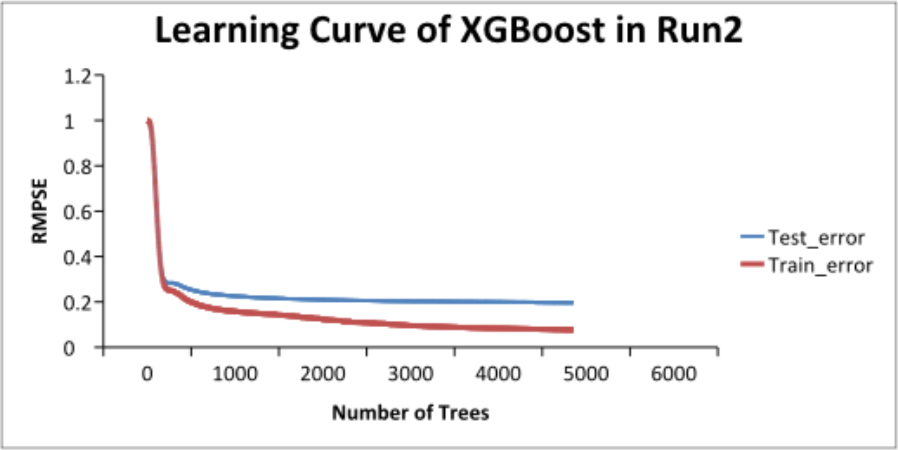
\includegraphics[width=\linewidth]{images/LearningCurve.png}
    \captionof{figure}{Learning Curve for 5000 tree model}
    \label{fig:LearningCurve}
\end{Figure}

Adding Competiton Age to our feature set did not improve our model on its own, but combining models (runs 3, 5, and 6) lead to a model with an improved RMSPE of 10.439\%, our best result.

\begin{table}[H]
\caption{Model Performance}
\centering
\begin{tabular}{lr}
\toprule
\cmidrule(r){1-2}
Model & RMSPE \\
\midrule
Gradient Boosting & 10.44\% \\
Random Forest &  11.98\% \\
Hidden Markov Model &  16.52\% \\
Predict Median Sales & 19.25\% \\
Recurrent Neural Nets &  24.88\% \\
\bottomrule
\end{tabular}
\end{table}

\section{Conclusion}

\indent \indent We found that though Hidden Markov Models and Recurrent Neural Networks are better in theory for time-series data, ensemble methods performed much better in practice. We believe this to be due to their robustness in black box optimization considering the data provided is unstructured and some features may not correlate well with sales.


%----------------------------------------------------------------------------------------
%	REFERENCE LIST
%----------------------------------------------------------------------------------------

\begin{thebibliography}{99} 

\bibitem{Figueredo:2009dg}
Figueredo, A.~J. and Wolf, P. S.~A. (2009).
\newblock Assortative pairing and life history strategy - a cross-cultural
  study.
\newblock {\em Human Nature}, 20:317--330.


\bibitem{Liaw:2002}
A. Liaw and M. Wiener (2002). 
\newblock Classification and Regression by randomForest.  
\newblock {\em R News}, 2(3):18--22.

\bibitem{Friedman}
 Friedman, Jerome H (2001).
 \newblock Greedy Function Approximation: A Gradient Boosting Machine.
 \newblock {\em The Annals of Statistics}, 29(5):1189-1232.
 
 \bibitem{Friedman2}
 Friedman, Jerome H (2002).
 \newblock Stochastic Gradient Boosting.
 \newblock {\em Computational Statistics \& Data Analysis}, 38(4):367-378.
 
 \bibitem{Samarasinghe}
 Samarasinghe, Sandhya (2006).
 \newblock Neural Networks for Applied Sciences and Engineering: From Fundamentals to Complex Pattern Recognition.
 \newblock {\em Auerbach Publications}
 
 \bibitem{Zucchini}
 Zucchini, Walter and MacDonald, Iain L. (2009)
 \newblock Hidden Markov Models for Time Series: An Introduction Using R (Chapman \& Hall/CRC Monographs on Statistics \& Applied Probability)
 \newblock {\em Chapman and Hall}

 
\end{thebibliography}

%----------------------------------------------------------------------------------------

\end{multicols}

\end{document}
